% ==== Type Punning done right ====
\section{Type Punning done right}

\begin{frame}{Possible (or not) approaches for type punning}
  People that type-pun, usually take one of the following approaches:
  \vfill

  \begin{itemize}
  \item Based on \texttt{union}
  \item Using \texttt{reinterpret\_cast} (sometimes combined w/ \texttt{std::launder})
  \item Use of \texttt{memcpy()}
  \item \texttt{std::bit\_cast}
  \item \texttt{std::start\_lifetime\_as}
  \end{itemize}

  \vfill
  \textbf{Some} of them lead to \textbf{UB in C++} (but otherwise correct in C)

  \begin{onlyenv}<2>
    \overlayLayer{
      You should also be aware of\ldots\vspace{1ex}
      \begin{itemize}
      \item \texttt{sizeof(char)}, \texttt{sizeof(int)}, etc., are platform-dependent.
        \begin{itemize}
        \item Use fixed-width integer types (e.g. \texttt{uint32\_t}) if appropriate
        \end{itemize}
        %
      \item ISO C++ requires \texttt{CHAR\_BIT} to be $\geq 8$; POSIX requires it to be $== 8$
      \end{itemize}
    }
  \end{onlyenv}
\end{frame}

\begin{frame}[fragile]{\texttt{union}-based}
  From \textit{[class.union.general]}: at most \textbf{one non-static member is active}; accessing non-active members of a \inlineCode{union} is \textbf{UB}!%
  \footnote{Accesses object whose lifetime has not begun.}.
  \footnote{Exception on next slide.}

  \begin{lstlisting}[style=c++]
    union {
      unsigned char c[sizeof(int)];
      int i;
    } u{ 0xff00ff00 }; // active member is 'i'

    `\pause`
    `\lsthl{u.c[0]; // UB!}`
  \end{lstlisting}

  \vfill
  \alert{IN GENERAL: DON'T!} -- It's legal in C, though.
\end{frame}

\begin{frame}[fragile]{\texttt{union}-based: THE ONLY EXCEPTION}
  \alert{BUT THERE'S ONE EXCEPTION!}
  \begin{block}{[class.union.general], p. 2, Note 1 says\ldots}
    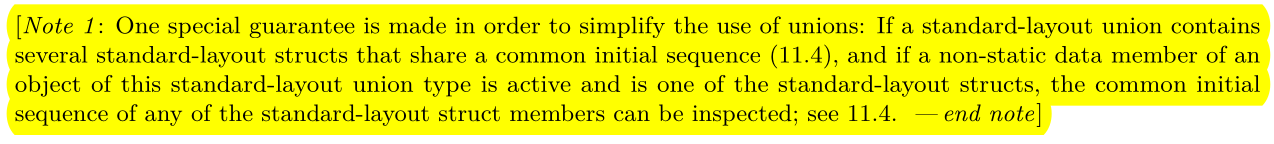
\includegraphics[width=\textwidth]{img/cplusplus_draft/class.union.general.2.Note_1.png}
  \end{block}

  \begin{onlyenv}<2>
    \overlayLayer{
      Again BSD sockets: \inlineCode{sockaddr} and \inlineCode{sockaddr\_in} have a common prefix\\[1em]
      \lstinputlisting[linerange={5-13},style=c++]{code/BSDsockets_union.cpp}
    }
  \end{onlyenv}
\end{frame}

\begin{frame}[fragile]{\texttt{reinterpret\_cast}-based}
  \inlineCode{reinterpret\_cast$<$T$>$(obj)} is guaranteed to be safe if
  \begin{itemize}
  \item Pointer $\leftrightarrow$ integral type (e.g. \texttt{uintptr\_t})

  \item Pointer-interconvertible \textit{[basic.compound], p. 5}:
    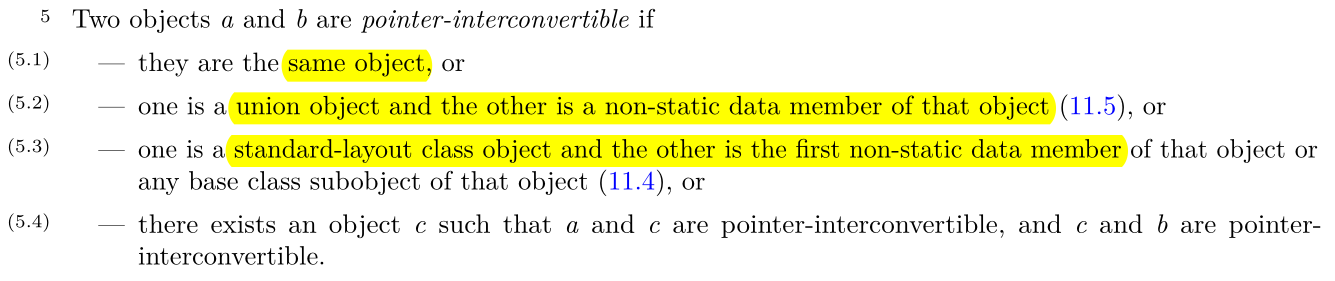
\includegraphics[width=\textwidth]{img/cplusplus_draft/basic.compound.5.png}

  \item Cast-to type is one of
    \begin{itemize}
    \item \texttt{char}, \texttt{unsigend char} or \texttt{std::byte}

    \item \texttt{decltype(obj)} (or its signed / unsigned type)
    \end{itemize}
  \end{itemize}

  \begin{onlyenv}<2>
    \overlayLayer{
      \begin{itemize}
      \item Don't do \texttt{reinterpret\_cast$<$float *$>$(\&an\_int)} (violates strict aliasing)
        %
      \item \alert{But even \texttt{reinterpret\_cast$<$unsigned char *$>$(\&something)} is not totally right}
        \begin{itemize}
        \item \alert{A \texttt{unsigned char []} object is not within its lifetime!}\footnote{Most compilers will do the right thing, but it's still UB!}
          %
        \item \href{https://www.open-std.org/jtc1/sc22/wg21/docs/papers/2025/p1839r7.html}{P1839R7} is supposed to fix that
          %
        \item What about \texttt{std::as\_bytes} / \texttt{std::as\_writable\_bytes} then? \facepalm
        \end{itemize}
      \end{itemize}
      %
      \rule{3em}{.1pt}\\
      \alert{Key idea:} pay attention to your \texttt{reinterpret\_cast}s; they are most likely UB (strict aliasing)!
    }
  \end{onlyenv}
\end{frame}

\begin{frame}{\texttt{std::launder}: w00t?}
  \inlineCode{std::launder} is\ldots
  \vfill

  \begin{itemize}
  \item According to \href{https://en.cppreference.com/w/cpp/utility/launder}{cppreference.com}: \\
    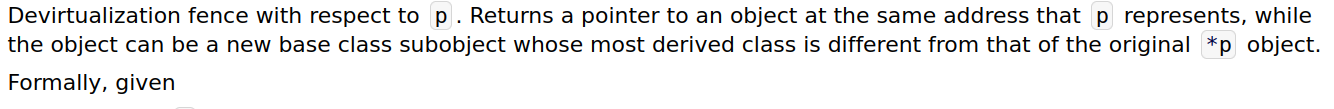
\includegraphics[width=\textwidth]{img/cppreference/ptr_launder.png}
    %
  \item According to ISO C++ wording: a pointer optimization barrier\\
    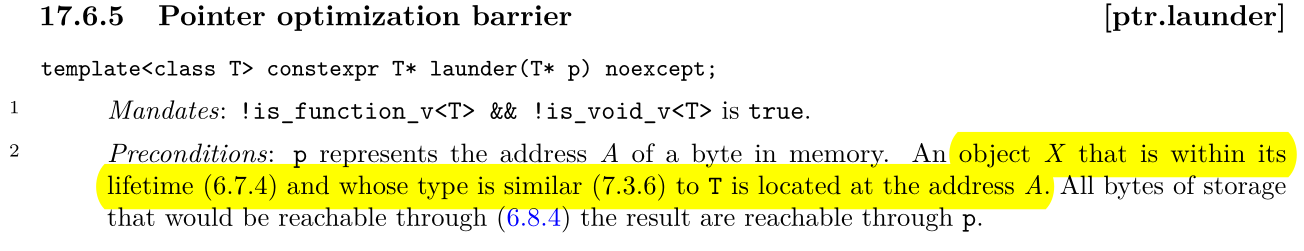
\includegraphics[width=\textwidth]{img/cplusplus_draft/ptr.launder.png}
  \end{itemize}

  \begin{onlyenv}<2>
    \tikz[remember picture,overlay]\node[at=(current page.center)]{\Huge\facepalm\facepalm\facepalm};
  \end{onlyenv}
\end{frame}

\begin{frame}{\texttt{std::launder}: pointer provenance}
  \begin{itemize}
  \item $Pointer \neq MemoryAddress$; an \textbf{address} is just the \textbf{value of a pointer}.

  \item In C++, \textbf{a pointer points to an object}. The compiler can make assumptions on the pointee.
  \end{itemize}

  Instead, think of a pointer as a pair
  \begin{equation*}
    \langle address, provenance \rangle
  \end{equation*}
  where $provenance$ determines which values can be reached through the pointer.
  \vfill
  \pause

  \begin{itemize}
  \item \textbf{Money laundering:} concealing the origin of money
    %
  \item \textbf{Pointer laundering:} update the provenance of a pointer, i.e. remove any assumptions on the pointee
  \end{itemize}

  \begin{onlyenv}<3>
    \overlayLayer{
      \begin{itemize}
      \item \alert{\bfseries Pre-conditions:}\\[1ex]
        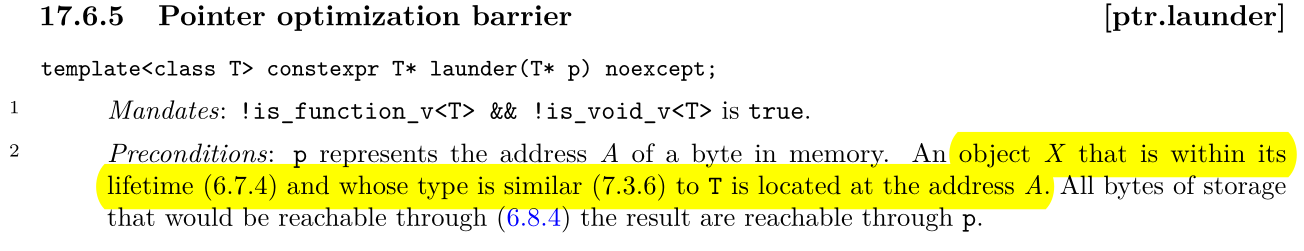
\includegraphics[width=.87\textwidth]{img/cplusplus_draft/ptr.launder.png}
        %
      \item Useful when replacing an object (reusing storage) that had \inlineCode{const} members or references
      \end{itemize}
    }
  \end{onlyenv}
\end{frame}

\begin{frame}[fragile]{\texttt{std::launder}: Example 1}
  \begin{lstlisting}[style=c++]
    uint32_t i = 42;
    float *fp = reinterpret_cast<float *>(&i);

    new (static_cast<void *>(&i)) float(12.34f);

    // std::cout << *fp << std::endl; // UB! 'fp' doesn't point to a 'float' object
    std::cout << `\lsthl{*std::launder(fp)}` << std::endl; // OK; 
  \end{lstlisting}
\end{frame}

\begin{frame}[fragile]{\texttt{std::launder}: Example 2}
  \lstinputlisting[linerange={5-19},style=c++]{code/std_launder.cpp}
\end{frame}

\begin{frame}[fragile]{\texttt{memcpy()} over (representation of) different object}
  \begin{lstlisting}[style=c++]
    uint32_t i = 42;

    float f;
    memcpy(&f, &i, sizeof(uint32_t)); // OK

    unsigned char c[sizeof(uint32_t)];
    memcpy(c, &i, sizeof(uint32_t)); // Also OK
  \end{lstlisting}

  \vspace{1em}
  \begin{center}
    Strict-aliasing [\OK]\hspace{4em}
    Alignment reqs. [\OK]\hspace{4em}
    Lifetime [\OK]\hspace{4em}
  \end{center}

  \begin{onlyenv}<2>
    \overlayLayer{
      \begin{itemize}
      \item \texttt{memcpy()} is optimized out where possible by major compilers \godbolt{https://godbolt.org/z/YnsrfWTjW}
      \end{itemize}
    }
  \end{onlyenv}
\end{frame}

\begin{frame}{\texttt{std::bit\_cast}}
  \begin{block}{\texttt{std::bit\_cast} \textit{[bit.cast], p. 1-2}}
    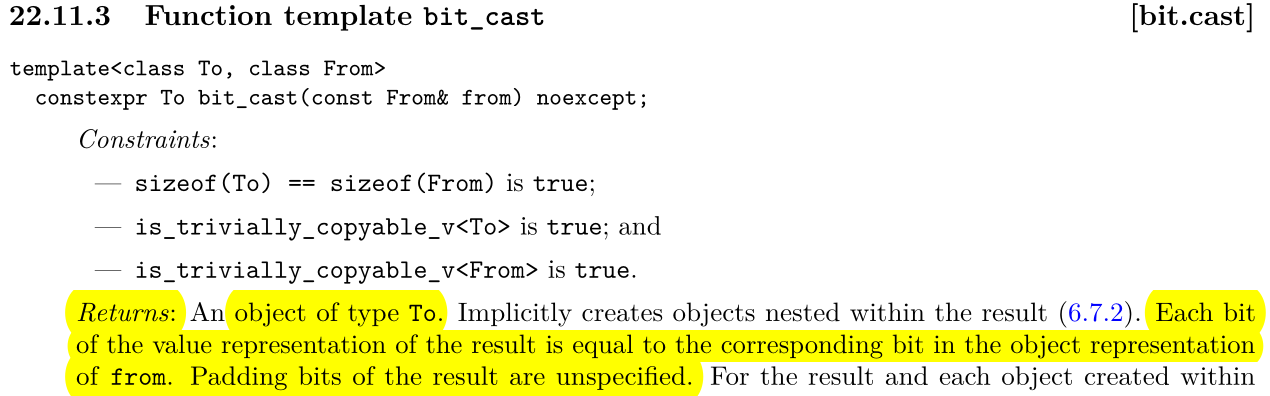
\includegraphics[width=\textwidth]{img/cplusplus_draft/bit.cast.png}
  \end{block}
\end{frame}

\begin{frame}[fragile]{\texttt{std::bit\_cast}: Example}
  \begin{lstlisting}[style=c++]
    float f = 42.0f;

    auto c = std::bit_cast<std::array<unsigned char, sizeof(float)>>(f);
    // Use the 'c' array
  \end{lstlisting}

  \vspace{1em}
  \begin{center}
    Strict-aliasing [\OK]\hspace{4em}
    Alignment reqs. [\OK]\hspace{4em}
    Lifetime [\OK]\hspace{4em}
  \end{center}

  \begin{onlyenv}<2>
    \overlayLayer{
      \begin{itemize}
      \item (Very) roughly speaking: ISO-CPP-blessed for the previous \texttt{memcpy()}
        %
      \item It's \inlineCode{constexpr}; optimized out where possible \godbolt{https://godbolt.org/z/ohMGr7dYW}
        %
      \item \alert{Note:} \texttt{std::bit\_cast$<$SomeType *$>()$} is simply \alert{WRONG}! (P0476R1)
      \end{itemize}
    }
  \end{onlyenv}
\end{frame}

\begin{frame}[fragile]{\texttt{std::start\_lifetime\_as} (C++23)}
  \begin{itemize}
  \item Explicit lifetime management (C++23)

  \item Starts lifetime of an object of the given type at the given address
    \begin{itemize}
    \item Underlying object representation is preserved
    \end{itemize}
  \end{itemize}

  \begin{lstlisting}[style=c++]
    uint32_t i = 42;
    float *f = std::start_lifetime_as<float>(&i);

    std::cout << *f << std::endl; // OK
  \end{lstlisting}
\end{frame}

\begin{frame}[fragile]{\texttt{std::start\_lifetime\_as} (C++23)}
  \begin{itemize}
  \item Recall the strict aliasing rule! No pair of objects of different type can be at same address!
    \begin{itemize}
    \item Thus, accessing \inlineCode{i} becomes UB!
    \end{itemize}
  \end{itemize}

  \pause
  \begin{lstlisting}[style=c++]
    uint32_t i = 42;
    float *f = std::start_lifetime_as<float>(&i);

    std::cout << *f << std::endl; // OK
    std::cout << i << std::endl; // `\lsthl{UB!}`
    std::start_lifetime_as<int>(&i);

    std::cout << i << std::endl; // `\lsthl{Still UB!}`
    std::cout << *std::launder(&i) << std::endl; // OK
  \end{lstlisting}
\end{frame}

\begin{frame}{In brief\ldots}
  Punning via \ldots{} is \ldots{}
  \begin{itemize}
  \item Based on \texttt{union} ~~\NotOK (note the exception)

  \item Using \texttt{reinterpret\_cast}
    \begin{itemize}
    \item Pointer $\leftrightarrow$ integral type: ~~\OK
    \item Pointer-interconvertible: ~~\OK
    \item To \texttt{char}-like type: ~~[Cast~\OK] [Deref~\question]
    \item \alert{Rest:} ~~\NotOK
    \end{itemize}

  \item Using \texttt{std::as\_bytes} / \texttt{std::as\_writable\_bytes} (C++20) ~~\OK~\question

  \item Use of \texttt{memcpy()} ~~\OK

  \item \texttt{std::bit\_cast} ~~\OK

  \item \texttt{std::start\_lifetime\_as} ~~\OK
  \end{itemize}
\end{frame}

\begin{frame}{What if $C++ \leq xx$}
  If $C++ \leq 23$\ldots
  \begin{itemize}
    \itemsep=1em
  \item Taking into account \linkButton{https://www.open-std.org/jtc1/sc22/wg21/docs/papers/2020/p0593r6.html}{P0593R6}, it may be implemented by using the special properties of \inlineCode{memmove()}

  \item The compiler infers the type of the object whose lifetime starts
  \end{itemize}

  \vfill
  If $C++ \leq 20$\ldots
  \begin{itemize}
    \itemsep=1em
  \item For \inlineCode{std::bit\_cast}: consider possible impl. described in \linkButton{https://en.cppreference.com/w/cpp/numeric/bit_cast}{cppreference.com}

  \item Or\ldots just use \inlineCode{memcpy()}
  \end{itemize}
\end{frame}
